\documentclass[fontsize=11pt]{article}
\usepackage{amsmath}
\usepackage[utf8]{inputenc}
\usepackage[margin=0.75in]{geometry}

\usepackage{xcolor}
\usepackage{setspace}
\usepackage{graphicx}
\usepackage[hidelinks,colorlinks=true,linkcolor=blue,citecolor=blue]{hyperref}

\newcommand{\blue}[1]{\textcolor{blue}{#1}}
\newcommand{\red}[1]{\textcolor{red}{#1}}
\newcommand{\link}[1]{\href{#1}{\blue{#1}}}

\definecolor{keywordred}{RGB}{255, 123, 114}
\definecolor{keywordorange}{RGB}{255, 166, 86}
\definecolor{keywordpurple}{RGB}{210, 168, 254}
\definecolor{commentblue}{RGB}{165, 214, 255}
\definecolor{noneblue}{RGB}{121, 192, 255}

\title{``Ram'' --- A Beginner's Introductory Programming Language Using Abstract Syntax Trees in Python}
\author{Will Assad, Ariel Chouminov, Ramya Chawla, Zain Lakhani}
\date{April 16, 2021}

\begin{document}

\maketitle

\section*{Problem Description and Research Question}
Modern programming languages are built using \blue{Abstract Syntax Trees (ASTs)}, a recursive data structure that represents written code \cite{david}. Programmers write code in the form of large strings, which are then parsed into ASTs in which the computer can understand and execute \cite{david, ASTs}. As humans, we often take this necessary translation for granted, given that we can simply read programs as text \cite{david}. The computer, however, interprets this text, translates it several times, and then produces an output with incredibly high speed. 

A programming language serves as an instrument to bridge the gap between machines and humans. Although the possibilities are seemingly limitless, a program is only as effective as the developer designs it to be. That is, the necessary tools to develop even the most complex programs are made available to one's disposal. However, with the vast number of nuances, it can be quite difficult for a beginner to indulge in the world of programming.

Programming languages present humans the opportunity to interact with computers in unique ways. One of these languages is \blue{Python}, a relatively easy scripting language to learn. While it has many advantages as a first programming language for new programmers, there are some key disadvantages. Mainly, it differs structurally from other programming languages in terms of indented blocks and variables that represent multiple data types. This means it offers beginner programmers an introduction into the world of programming while making their transition into other languages quite difficult. 

The other problem with introducing programming to new students of Computer Science is getting them to understand what a particular syntax represents in English. The intuition behind writing certain lines of code can hide from those who lack experience. For example, there is no obvious reason why the line of Python code \texttt{print([(x, x \% 2 == 0) for x in range(10)])} should display a list of numbers from 0 to 9 and whether or not they are even. Hence, \blue{\textbf{the goal of this project is to create a programming language (Ram) that is easily translatable to English and helps better prepare beginner programmers to use other programming languages.}} That is, we're looking to provide our users with the ability to convert basic English sentences, following the syntax of our language, into lines of Ram code.

\section*{Computational Plan}

Before diving directly into the code and our plan of implementation, we will clearly define all the syntactical structures of Ram code. As previously mentioned, an important feature is the readability of this code and the fluency with which it can be translated to English. \hyperlink{tab1}{Table 1} contains various expressions in Python with a side-by-side comparison of how they can be expressed following the syntax of Ram code.

\begin{center}
    \begin{spacing}{1.1}
    
        \hypertarget{tab1}{}
    
        \begin{tabular}{|l|l|} 
             \hline
             
             \blue{Python Syntax} & \blue{Ram Syntax} \\ 
             
             \hline
             \texttt{for x in \red{range(5)}:} & \texttt{loop with x \red{from 0 to 4} \{ } \\ 
             \quad \quad \texttt{print(x)} & \quad \quad  \texttt{display x} \\
              & \} \\
             
             \hline
             
             \texttt{\red{x} = 5} & \texttt{\red{set integer} x to 5} \\
             
             \hline
             
             \texttt{\red{letters} = `hello'} & \texttt{\red{set text} letters to ``hello''} \\
             
             \hline
             
        \end{tabular}
             
        \begin{tabular}{|l|l|} 
             \hline
             
             \texttt{\red{def} f(x:\,int) -> None:} & \texttt{\red{new function} f takes (x) \{ } \\
             \quad \quad \texttt{x = x - 5} & \quad \quad \texttt{\red{reset x} to x - 5} \\
             \quad \quad \texttt{print(x)} & \quad \quad \texttt{display x} \\
              & \} \\
              
             \hline
             
             \texttt{\red{var1} = 10} & \texttt{\red{set integer} var1 to 10} \\ 
             \texttt{\red{var2} = f(8) } &               \texttt{\red{set integer} var2 to f[x=8]} \\
             
             \quad \quad & \quad \quad \\
             
             \texttt{\red{if} var1 \red{==} var2:} & \texttt{\red{if} (var1) \red{is} (var2) \{ } \\
             
             \quad \quad \texttt{print(`They are equal!')} & \quad \quad \texttt{display ``They are equal!''} \\
             
             \texttt{\red{elif} (var1 + var2) \red{==} 5:} & \texttt{\} \red{else if} (var1 + var2) \red{is} (5) \{ } \\
             
             \quad \quad \texttt{print(`Equals 5')} & \quad \quad \texttt{display ``Equals 5''} \\

             \quad \quad \texttt{var1 = 4} & \quad \quad \texttt{\red{reset var1} to 4} \\
             
             \texttt{\red{else}: } & \texttt{\} \red{else} \{} \\
             
             \quad \quad \texttt{print(`Nothing happened.')} & \quad \quad \texttt{display ``Nothing happened.''} \\
              
             \quad \quad & \texttt{\}} \\
             
             \hline 
             
             \texttt{\red{def} compute(x:\,int, y:\,int) -> int:} & \texttt{\red{new function} f takes (x,y) \{ } \\
             \quad \quad \texttt{x = x + y} & \quad \quad \texttt{\red{reset x} to x + y} \\
             \quad \quad \texttt{\red{return} x} & \quad \quad \texttt{\red{send back} x} \\
              & \} \\
              
             \hline
        \end{tabular}
    
    \end{spacing}
    
    $ $
    
    \small{\textcolor{blue}{Table 1}: Comparison of Python and Ram Syntax}
    
\end{center}

Our program consists of three main parts. Initially, we begin by defining various statements and expressions in Python such as for-loops, functions, if-statements, assignment statements, and print statements. We define these statements through the use of Abstract Syntax Trees (\hyperlink{fig1}{Figure 1}). We define an abstract class representing a statement, \texttt{Statement}, and an abstract subclass representing an expression, \texttt{Expr}\footnote{These two abstract classes and subclasses such as \texttt{If}, \texttt{BoolOp}, and \texttt{Loop} are credited to the \emph{CSC111} notes \cite{david}.}.

$ $

\hypertarget{fig1}{}

\texttt{\textcolor{keywordred}{class} \textcolor{keywordorange}{Statement}:}

\quad\quad \texttt{\textcolor{commentblue}{"""An abstract class representing a Python statement.}}

\quad\quad{\texttt{\textcolor{commentblue}{"""}}}

\quad\quad\texttt{\textcolor{keywordred}{def} \textcolor{keywordpurple}{evaluate}(self, env: \textcolor{keywordorange}{dict[str, Any]}) -> Optional[Any]:}

\quad\quad\texttt{"""Evaluate this statement with the given environment."""}

\quad\quad \quad\quad \texttt{\textcolor{keywordred}{raise} \textcolor{keywordorange}{NotImplementedError}}

$ $

\texttt{\textcolor{keywordred}{class} \textcolor{keywordorange}{Expr}:}

\quad\quad \texttt{\textcolor{commentblue}{"""An abstract class representing a Python expression.}}

\quad\quad{\texttt{\textcolor{commentblue}{"""}}}

\quad\quad\texttt{\textcolor{keywordred}{def} \textcolor{keywordpurple}{evaluate}(self, env: \textcolor{keywordorange}{dict[str, Any]}) -> Optional[Any]:}

\quad\quad\texttt{"""Evaluate this statement with the given environment."""}

\quad\quad \quad\quad \texttt{\textcolor{keywordred}{raise} \textcolor{keywordorange}{NotImplementedError}}

$ $

\begin{center}
    \small{\textcolor{blue}{Figure 1}: \texttt{Statement} and \texttt{Expr} Abstract Classes}
\end{center}

ASTs are a form of trees since a \texttt{Statement} can be composed of many \texttt{Expr}'s which can also be composed of many different other \texttt{Expr}'s, which represent subtrees. For example, a binary operation expression \texttt{BinOp(Expr)} is defined in terms of a left \texttt{Expr} and a right \texttt{Expr} as seen in \hyperlink{fig2}{Figure 2}. This allows for any form of nesting, provided that the left and right subtrees evaluate to  floating-point values. All other ASTs have a similar structure, being composed of other statements and expressions.



\begin{center}
    \hypertarget{fig2}{}

    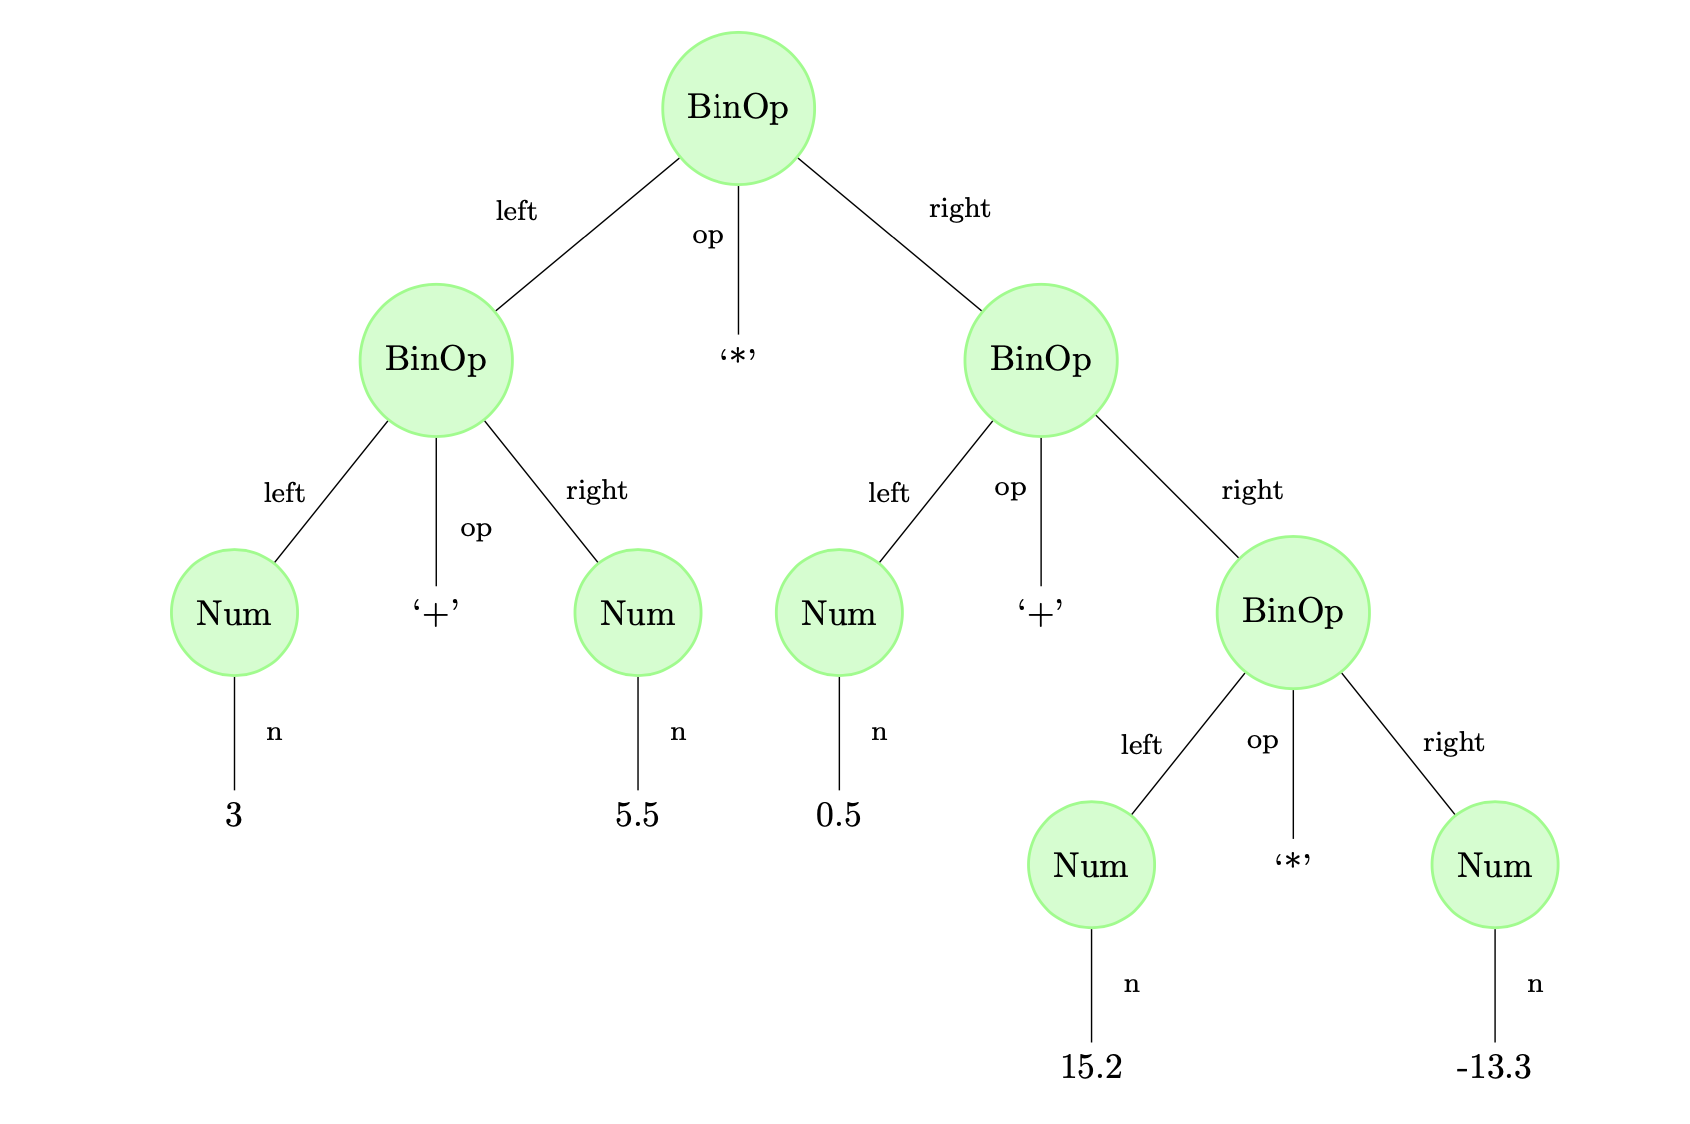
\includegraphics[scale=0.4]{binop2.png}
    
    \small{\textcolor{blue}{Figure 2}: \texttt{BinOp} Tree Structure}
    
    $ $
\end{center}

We as humans take for granted the complexity in interpreting the context of plain text. We read from left to right, and process text with ease. A computer, however, must convert the plain text into the deeply nested structures as seen in \hyperlink{fig2}{Figure 2}. This is the process of parsing. 

As previously mentioned, parsing, within the context of programming, is the process of analyzing a string of symbols and or words that are presented in either natural language, computer language, or data structures \cite{def}. Similar to Python, the code written by our users will initially be processed as the basic data types --- strings, booleans, and integers. However, from there, we begin to parse the data into the ASTs. Since parsing is the most difficult and technically demanding component of our project, we decided to divide and conquer. Parsing numbers, variables, and everything else in between was done separately in three main steps:

\begin{enumerate}
    \item \blue{Read in the \texttt{.ram} file as a list of tuples.}
    
    The \texttt{.ram} file is read in as a list of tuples where each tuple contains the line and the line number. 
    
    \item \blue{Recursively create the nested block structure.}
    
    In \texttt{parsing.py}, we introduced an abstract class \texttt{Block} (\hyperlink{fig3}{Figure 3}) which has three sub-classes --- \texttt{Loop}, \texttt{Function}, and \texttt{If}. A complicated recursive algorithm \texttt{make\_child} that runs in \texttt{Block.\_\_init\_\_} creates the relevant nested structure. The function determines the block type of the caller and creates a new specific block instance. The newly created block recursively parses through all of its children, which runs through the same process as the parent. The parent class assigns its caller a new sub-class type (for example a Loop Block), so that when the block is parsed, the parsing specific to that block type is executed. Similar to \texttt{Statement} and \texttt{Expr}, these classes and sub-classes are used to create a nested structure. The use of these classes allows us to recursively parse each block of code. 
    
    \item \blue{Recursively parse the nested block structure.}
    
     Each type of \texttt{Line} and child of \texttt{Block} has its own \texttt{parse} method which recursively creates an AST. For example, \texttt{IfBlock.parse} would return the AST \texttt{If(Statement)}.
    
    \item \blue{Evaluate the resulting ASTs.}
    
    As described in \hyperlink{fig1}{Figure 1}, each AST has an \texttt{evaluate} method. For example, \texttt{BinOp.evaluate} would return a floating point value, as represented in Python.
    
\end{enumerate}

$ $

\hypertarget{fig3}{}

\texttt{\textcolor{keywordred}{class} \textcolor{keywordorange}{Block}:}

\quad\quad \texttt{\textcolor{commentblue}{"""A block of Ram code to parse.}}

\quad\quad{\texttt{\textcolor{commentblue}{"""}}}

\quad\quad\texttt{\textcolor{keywordred}{def} \textcolor{keywordpurple}{parse}(self) -> Statement:}

\quad\quad\texttt{"""Parse a block of Ram code."""}

\quad\quad \quad\quad \texttt{\textcolor{keywordred}{raise} \textcolor{keywordorange}{NotImplementedError}}

$ $
\begin{center}

    \small{\textcolor{blue}{Figure 3}: \texttt{Block} Abstract Class}
\end{center}

Our language is intended to support simple arithmetic expressions, including the use of brackets. Regardless of the number of smaller computations that are nested within any binary operation, we need to evaluate the expression in terms of the order of operations. We were able to successfully implement very complex recursive algorithms such as \texttt{lexify} and \texttt{pedmas} in \textit{parsing/parse\_numeric.py}. This being said, recursion was an essential tool in many algorithms; without it, we would have great difficulty locating and keeping track of various blocks of code.

To give an example of this process, let's run through the specific algorithm for parsing this line of Ram code:

\begin{center}
    \texttt{\red{set integer} var1 to 4 * 3 + (8 - 4 * 2)}
\end{center}

This line is read in as a tuple consisting of the line itself as a string and the corresponding line number in the enclosing file. The keyword \texttt{set} is detected, meaning the line is to be parsed as a variable assignment statement. The keyword \texttt{integer} is detected, meaning the line is to be parsed more specifically as a numerical value. The variable name, \texttt{var1}, is stored and the numeric expression \texttt{4 * 3 + (8 - 4 * 2)} is run through the \texttt{lexify} algorithm. This algorithm is fairly complex, using recursion to create the relevant nesting structure around the binary operations, following the mathematical order of operations. Once this process is finished, \texttt{var1} is assigned to the \texttt{BinOp} returned by the \texttt{lexify} algorithm. Finally, the statement is evaluated and the environment is updated to contain the new variable.

\noindent The intuition is to take blocks of code and separate them into loop blocks, if blocks, and function blocks. Then the body portion of those blocks can contain nested blocks within, and this forms the nested structure we addressed earlier. Once these blocks are parsed, the program is able to treat them as functions and can accurately identify and interpret each statement of code. 

We also need to ensure that the nesting of the blocks occurs in the correct order. Which brings us to the \texttt{process\_ram} function in \texttt{process.py}. With the assistance of a helper function, we're able to use \texttt{process\_ram} to take in chunks of Ram code as a list of tuples in the form: \texttt{[($<$line$>$, $<$line number$>$), \dots]} and return a list which correctly nests the blocks provided. Therefore, this function essentially transform the data into a nested structure in an accurate manner. Further, the recursive nature of this function is directly associated with trees, as it can be viewed as a non-binary tree where each node has one child and each child represents a recursive call. 

As a result of the combination of these AST's, we are able to successfully create an interactive component and allow the user to freely experiment with Ram code and even build simplistic programs. The overarching theme of simplistic, introductory programming is obtained by following a parsing similar to that of Python, but with a more surface level depth in terms of the features and capabilities of the program. But what the program lacks in sophistication, it makes up for with directness, as users are now able to follow clear syntax guidelines to convert near-standard English convention sentences into actual lines of code. 

For the libraries, we used \texttt{sys}, \texttt{os} and \texttt{platform}, which all come packaged with python and do not require any additional installation. We used \texttt{sys} to read the command line argument when calling \texttt{ram <filepath>.ram} in order to get the file path in the \texttt{verify\_file} function in \texttt{process.py}. In \texttt{install.py}, \texttt{platform} and \texttt{os} are used in the \texttt{InstallRam} class. An alias that links to an executable \texttt{main.py} is created at \texttt{usr/local/bin/ram} using \texttt{os}. This is only done (using \texttt{platform}) provided the platform is Darwin.


\section*{Running the Program}
\subsection*{Using MacOS}
    \begin{itemize}
        \item \blue{Python Console}
        \begin{itemize}
            \item You can write a new \texttt{.ram} file in any text editor. We even defined custom syntax highlighting for \texttt{*.ram} files in PyCharm (see images below)! 
            
            \item Run main.py
            
            \item You will be prompted to enter the file path of the .ram file to run.
            
            \bigskip
            
            \bigskip
            
        \end{itemize}
        \item \blue{Terminal}
        \begin{itemize}
            \item Open Terminal and type \texttt{which python} or \texttt{which python3} (depending on the version installed).
            
            \begin{center}
                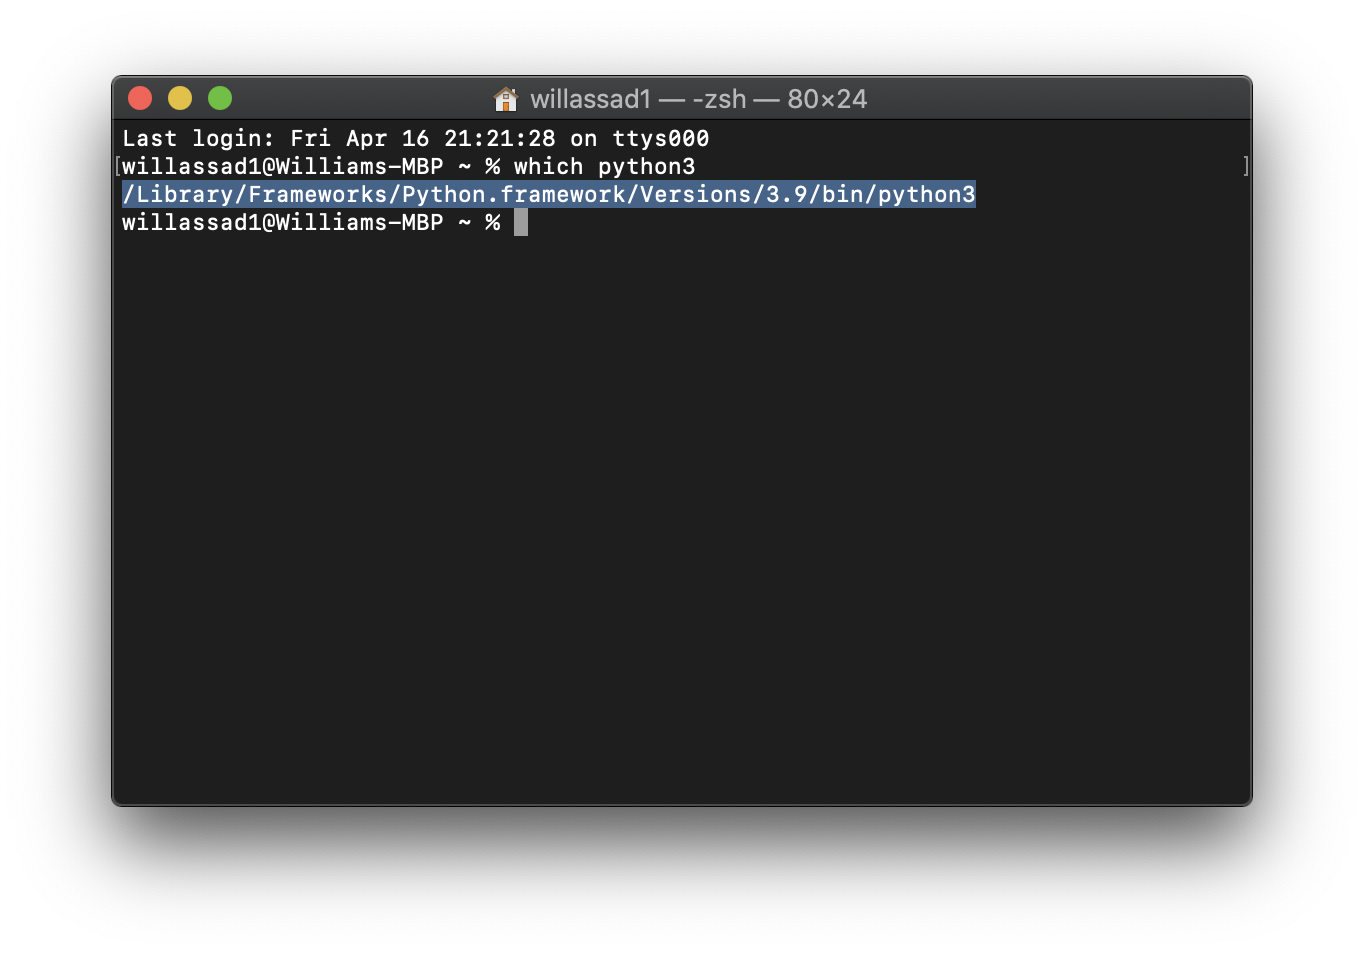
\includegraphics[scale=0.42]{terminal1.png}
            \end{center}
            
             \item Copy the result and then open \texttt{main.py} and paste the result after the \texttt{!\#}.
             
             \begin{center}
                 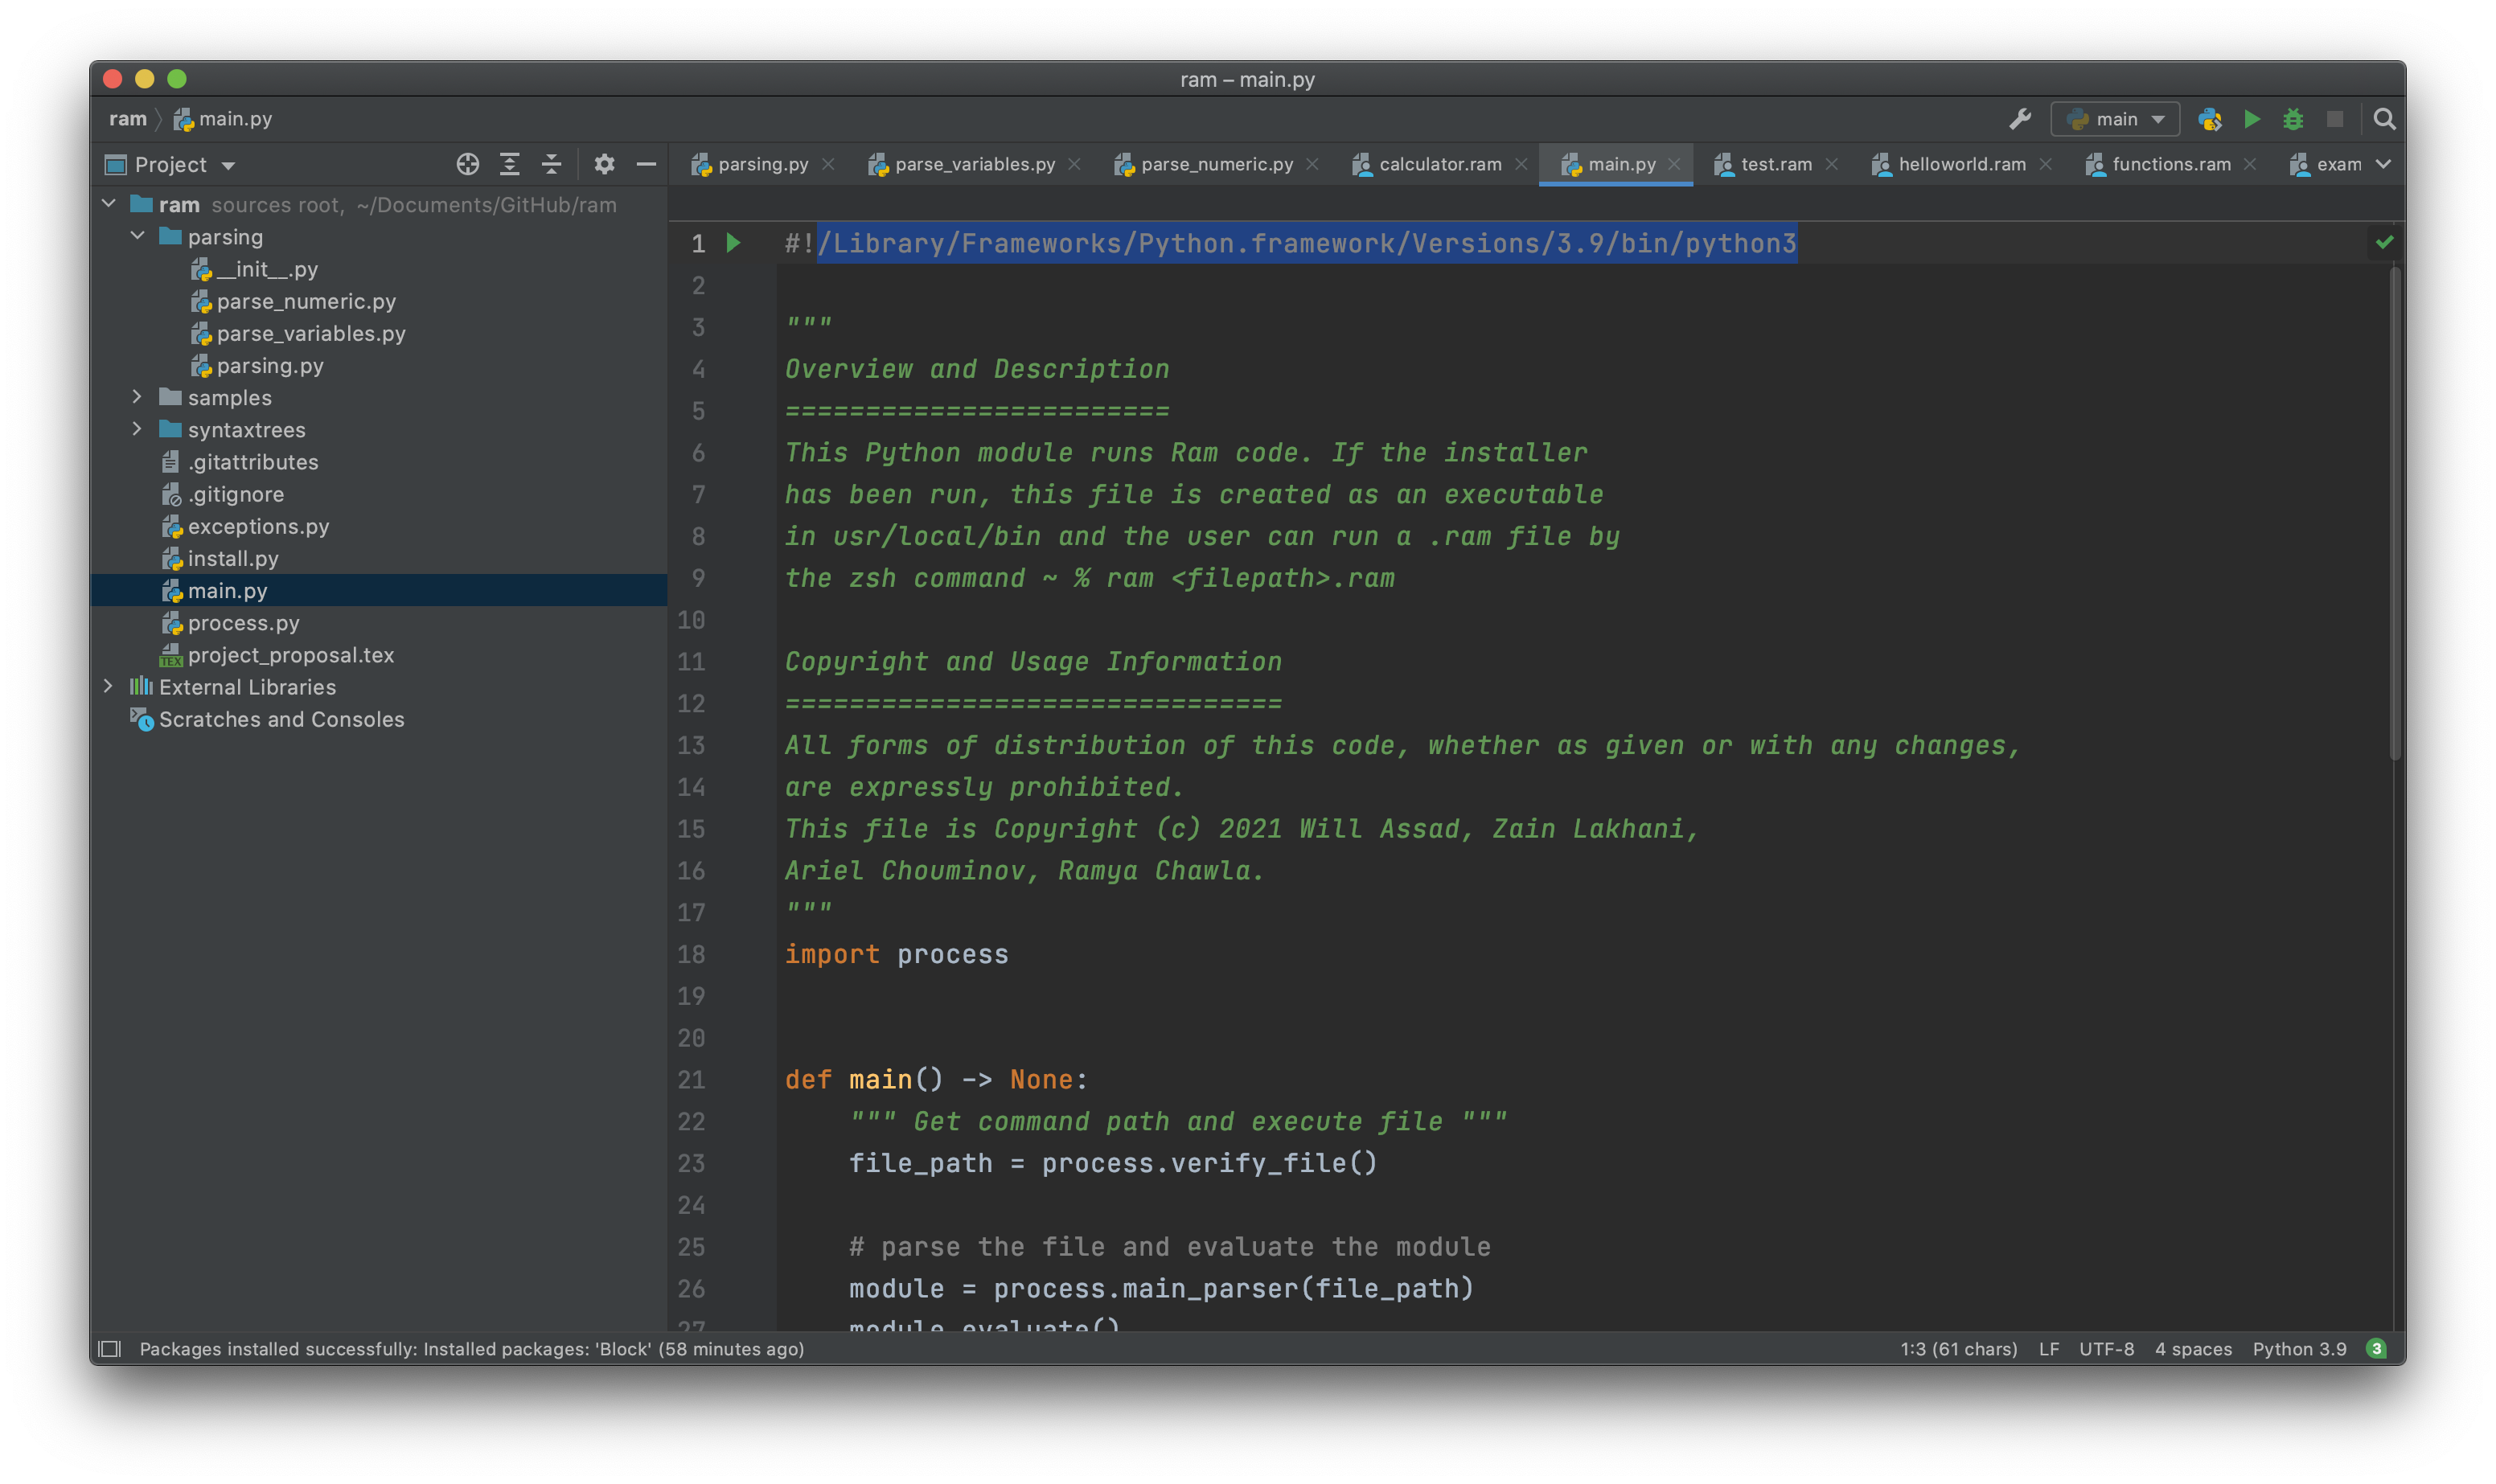
\includegraphics[scale=0.2]{terminal4.png}
             \end{center}
            
            \item Navigate to the main \texttt{ram} program directory (wherever it is stored).
            
            \begin{center}
                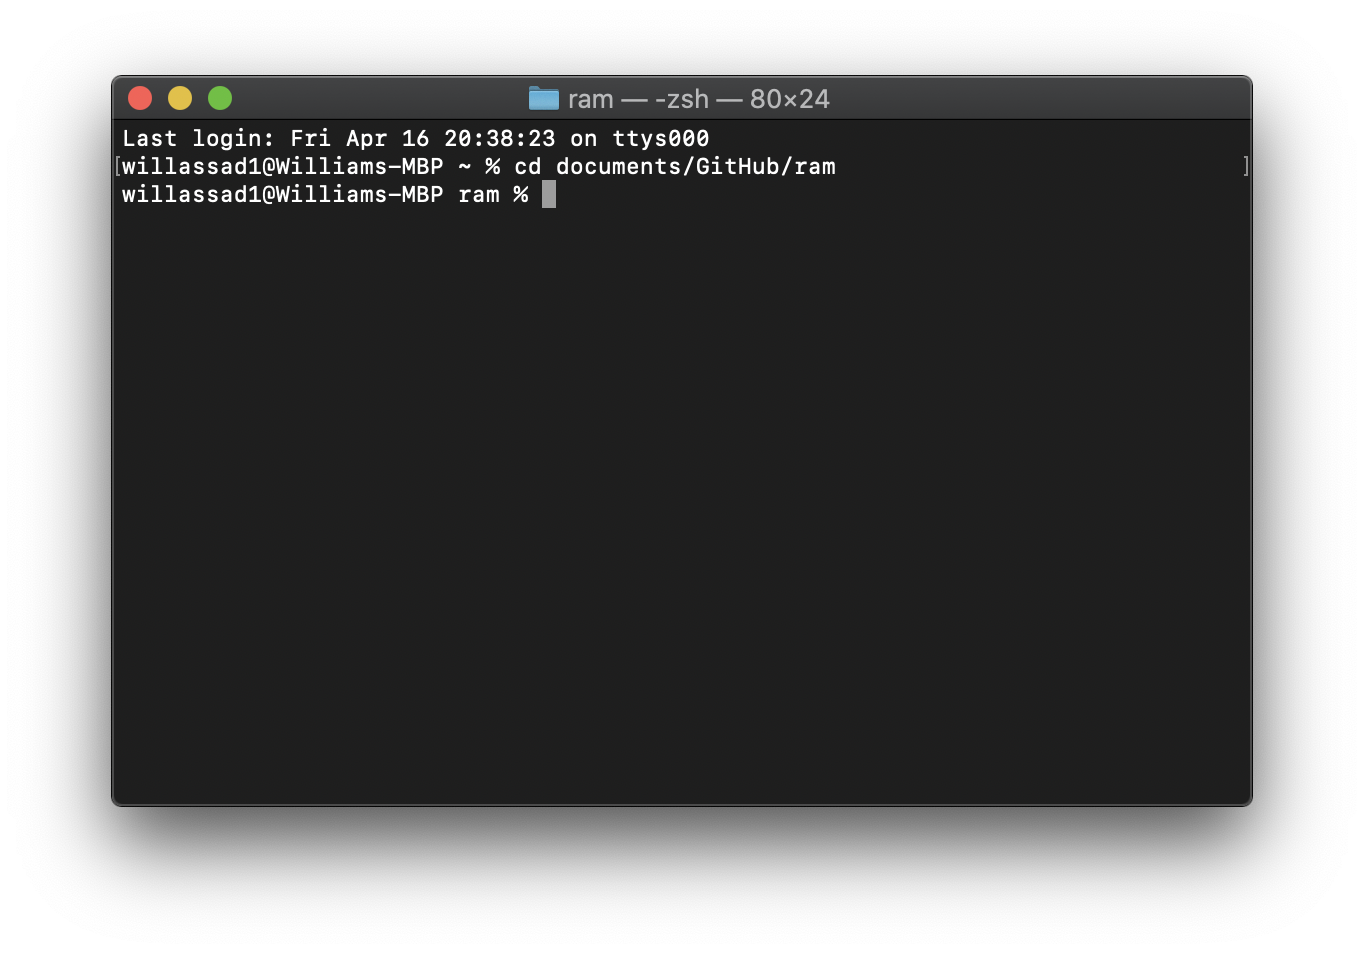
\includegraphics[scale=0.42]{terminal2.png}
            \end{center}
            
            \item Now run the command \texttt{python install.py} or \texttt{python3 install.py} (depending on version used).
            
            \begin{center}
                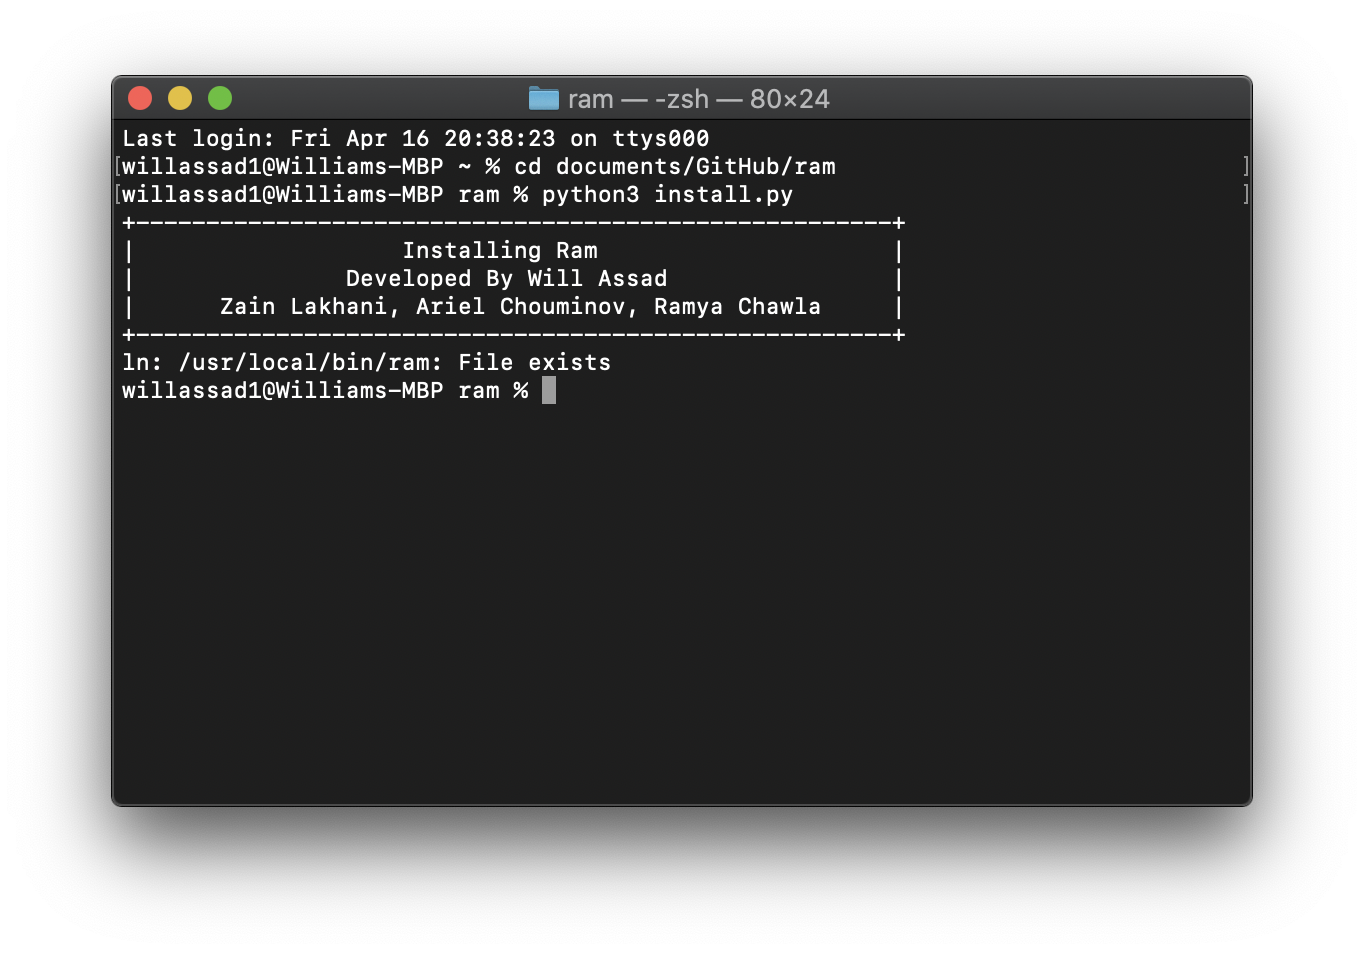
\includegraphics[scale=0.42]{terminal3.png}
            \end{center}
            
            \item You can now write a new \texttt{.ram} file in any text editor. We even defined custom syntax highlighting for \texttt{*.ram} files in PyCharm!
            
            \begin{center}
                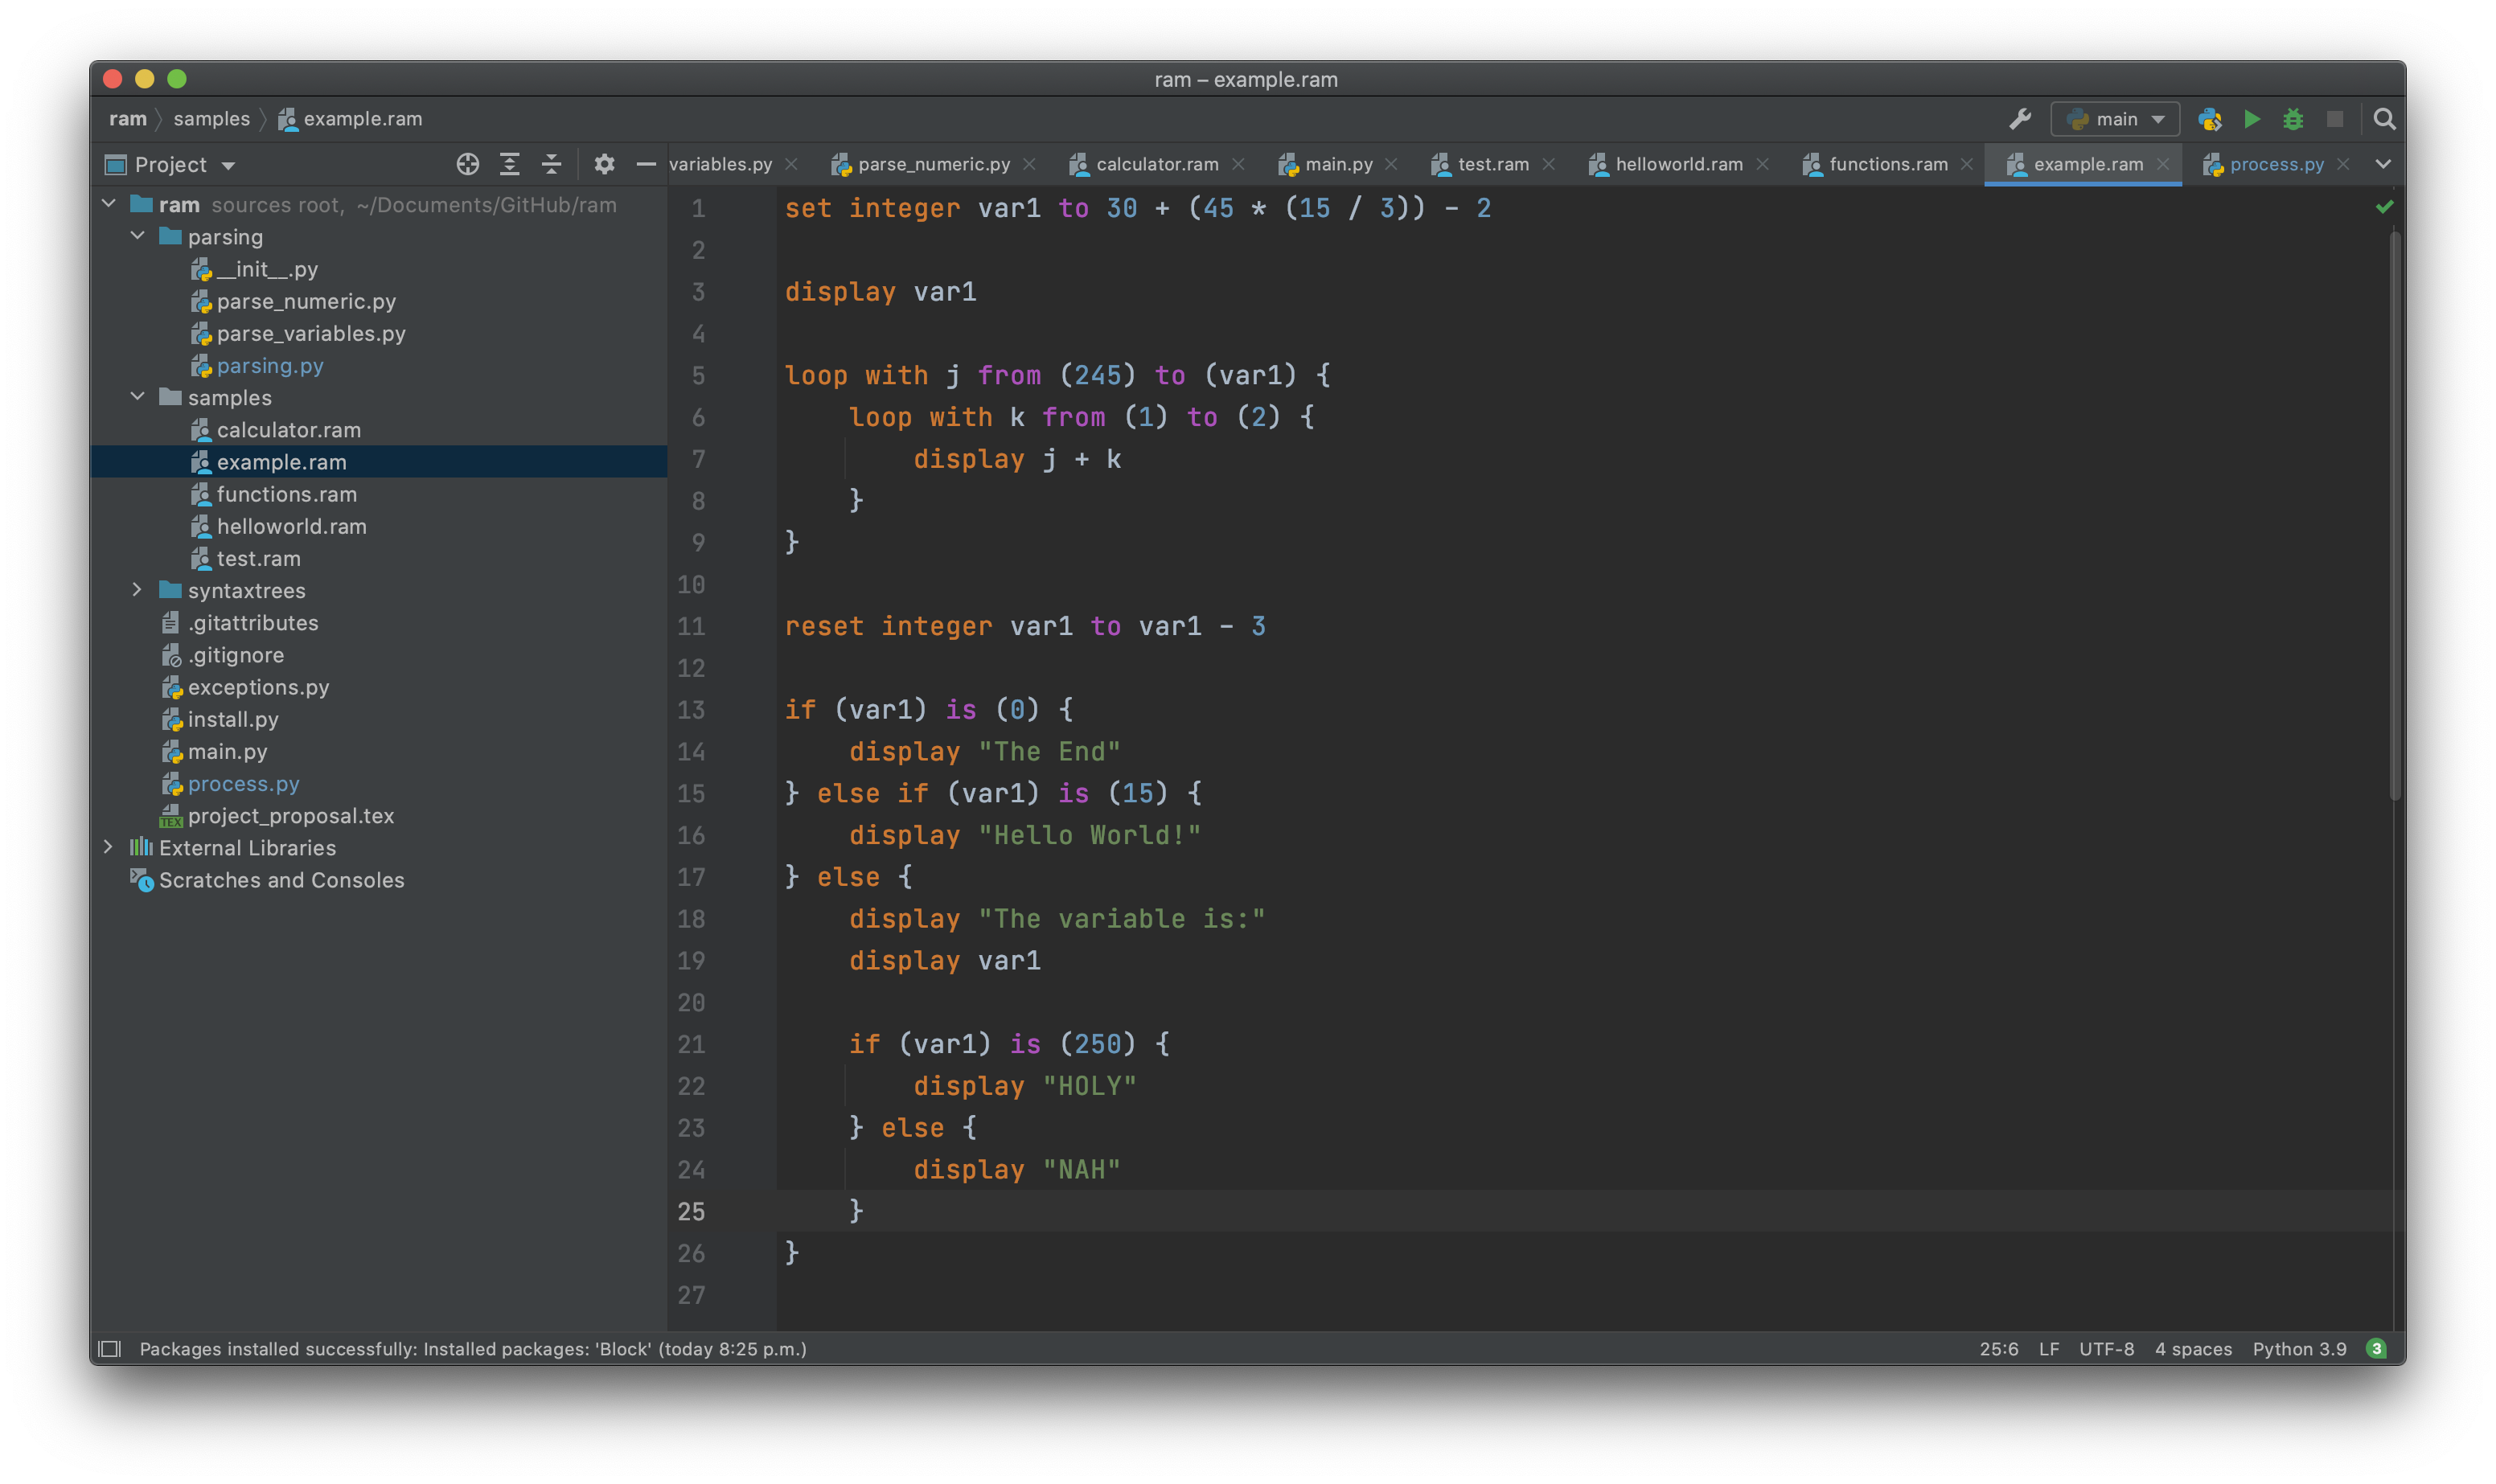
\includegraphics[scale=0.2]{terminal5.png}
            \end{center}
            
            \item Then run the file using the command \texttt{ram <filepath>.ram} or just \texttt{ram}.
            
            \begin{center}
                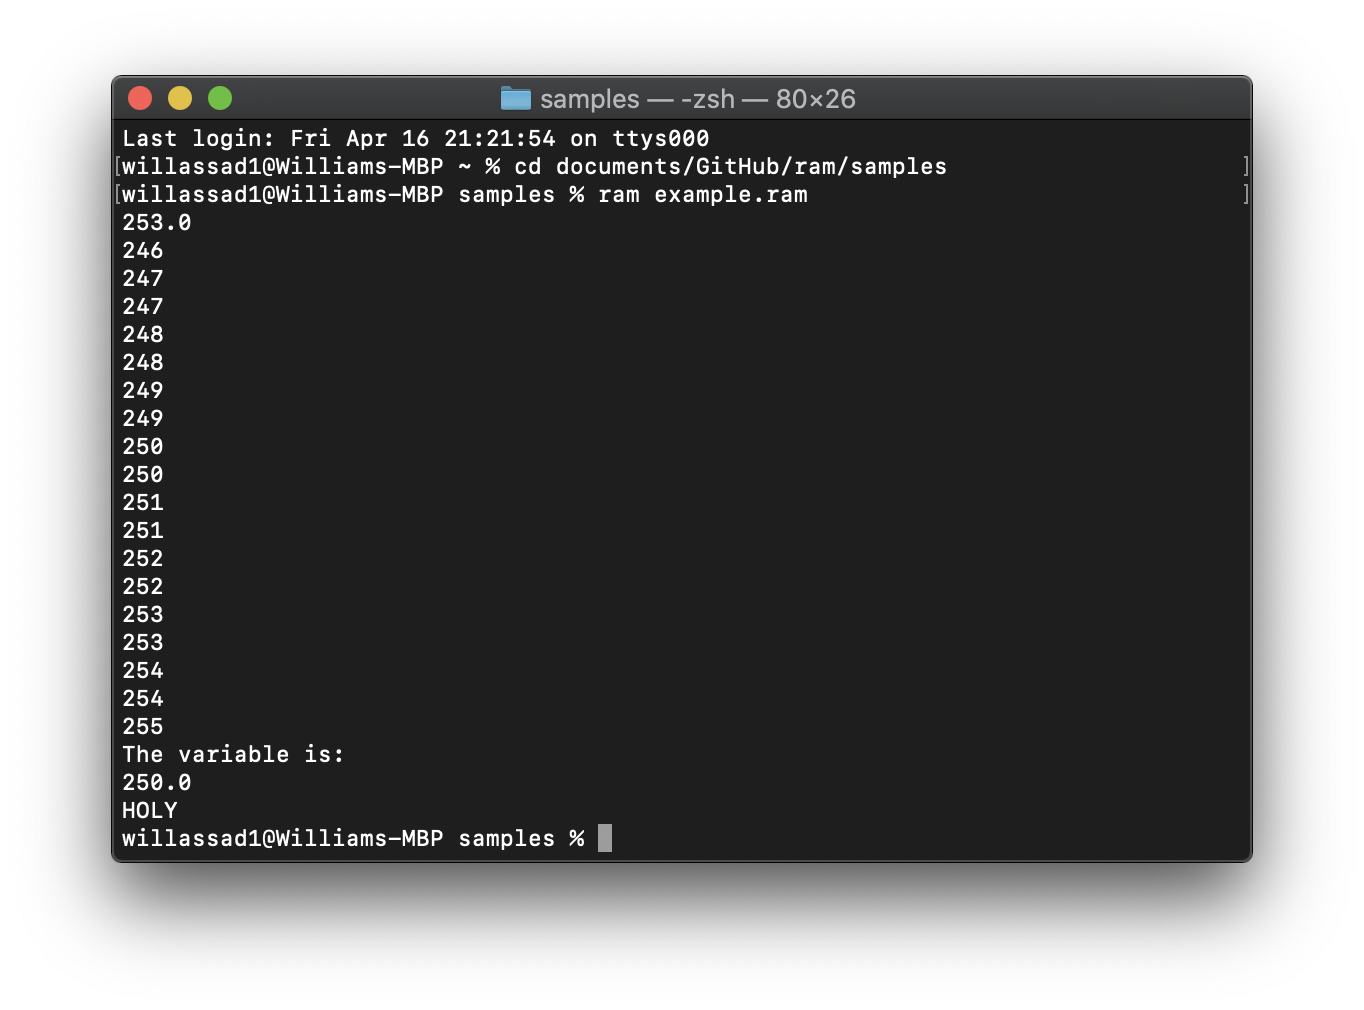
\includegraphics[scale=0.42]{terminal6.png}
            \end{center}
            
        \end{itemize}
    \end{itemize} 

\subsection*{Using Windows}

\emph{Note:} only python console is supported in Windows.

  \begin{itemize}
        \item \blue{Using Python Console}
        \begin{itemize}
            \item You can write a new \texttt{.ram} file in any text editor. We even defined custom syntax highlighting for \texttt{*.ram} files in PyCharm!
            
            \begin{center}
                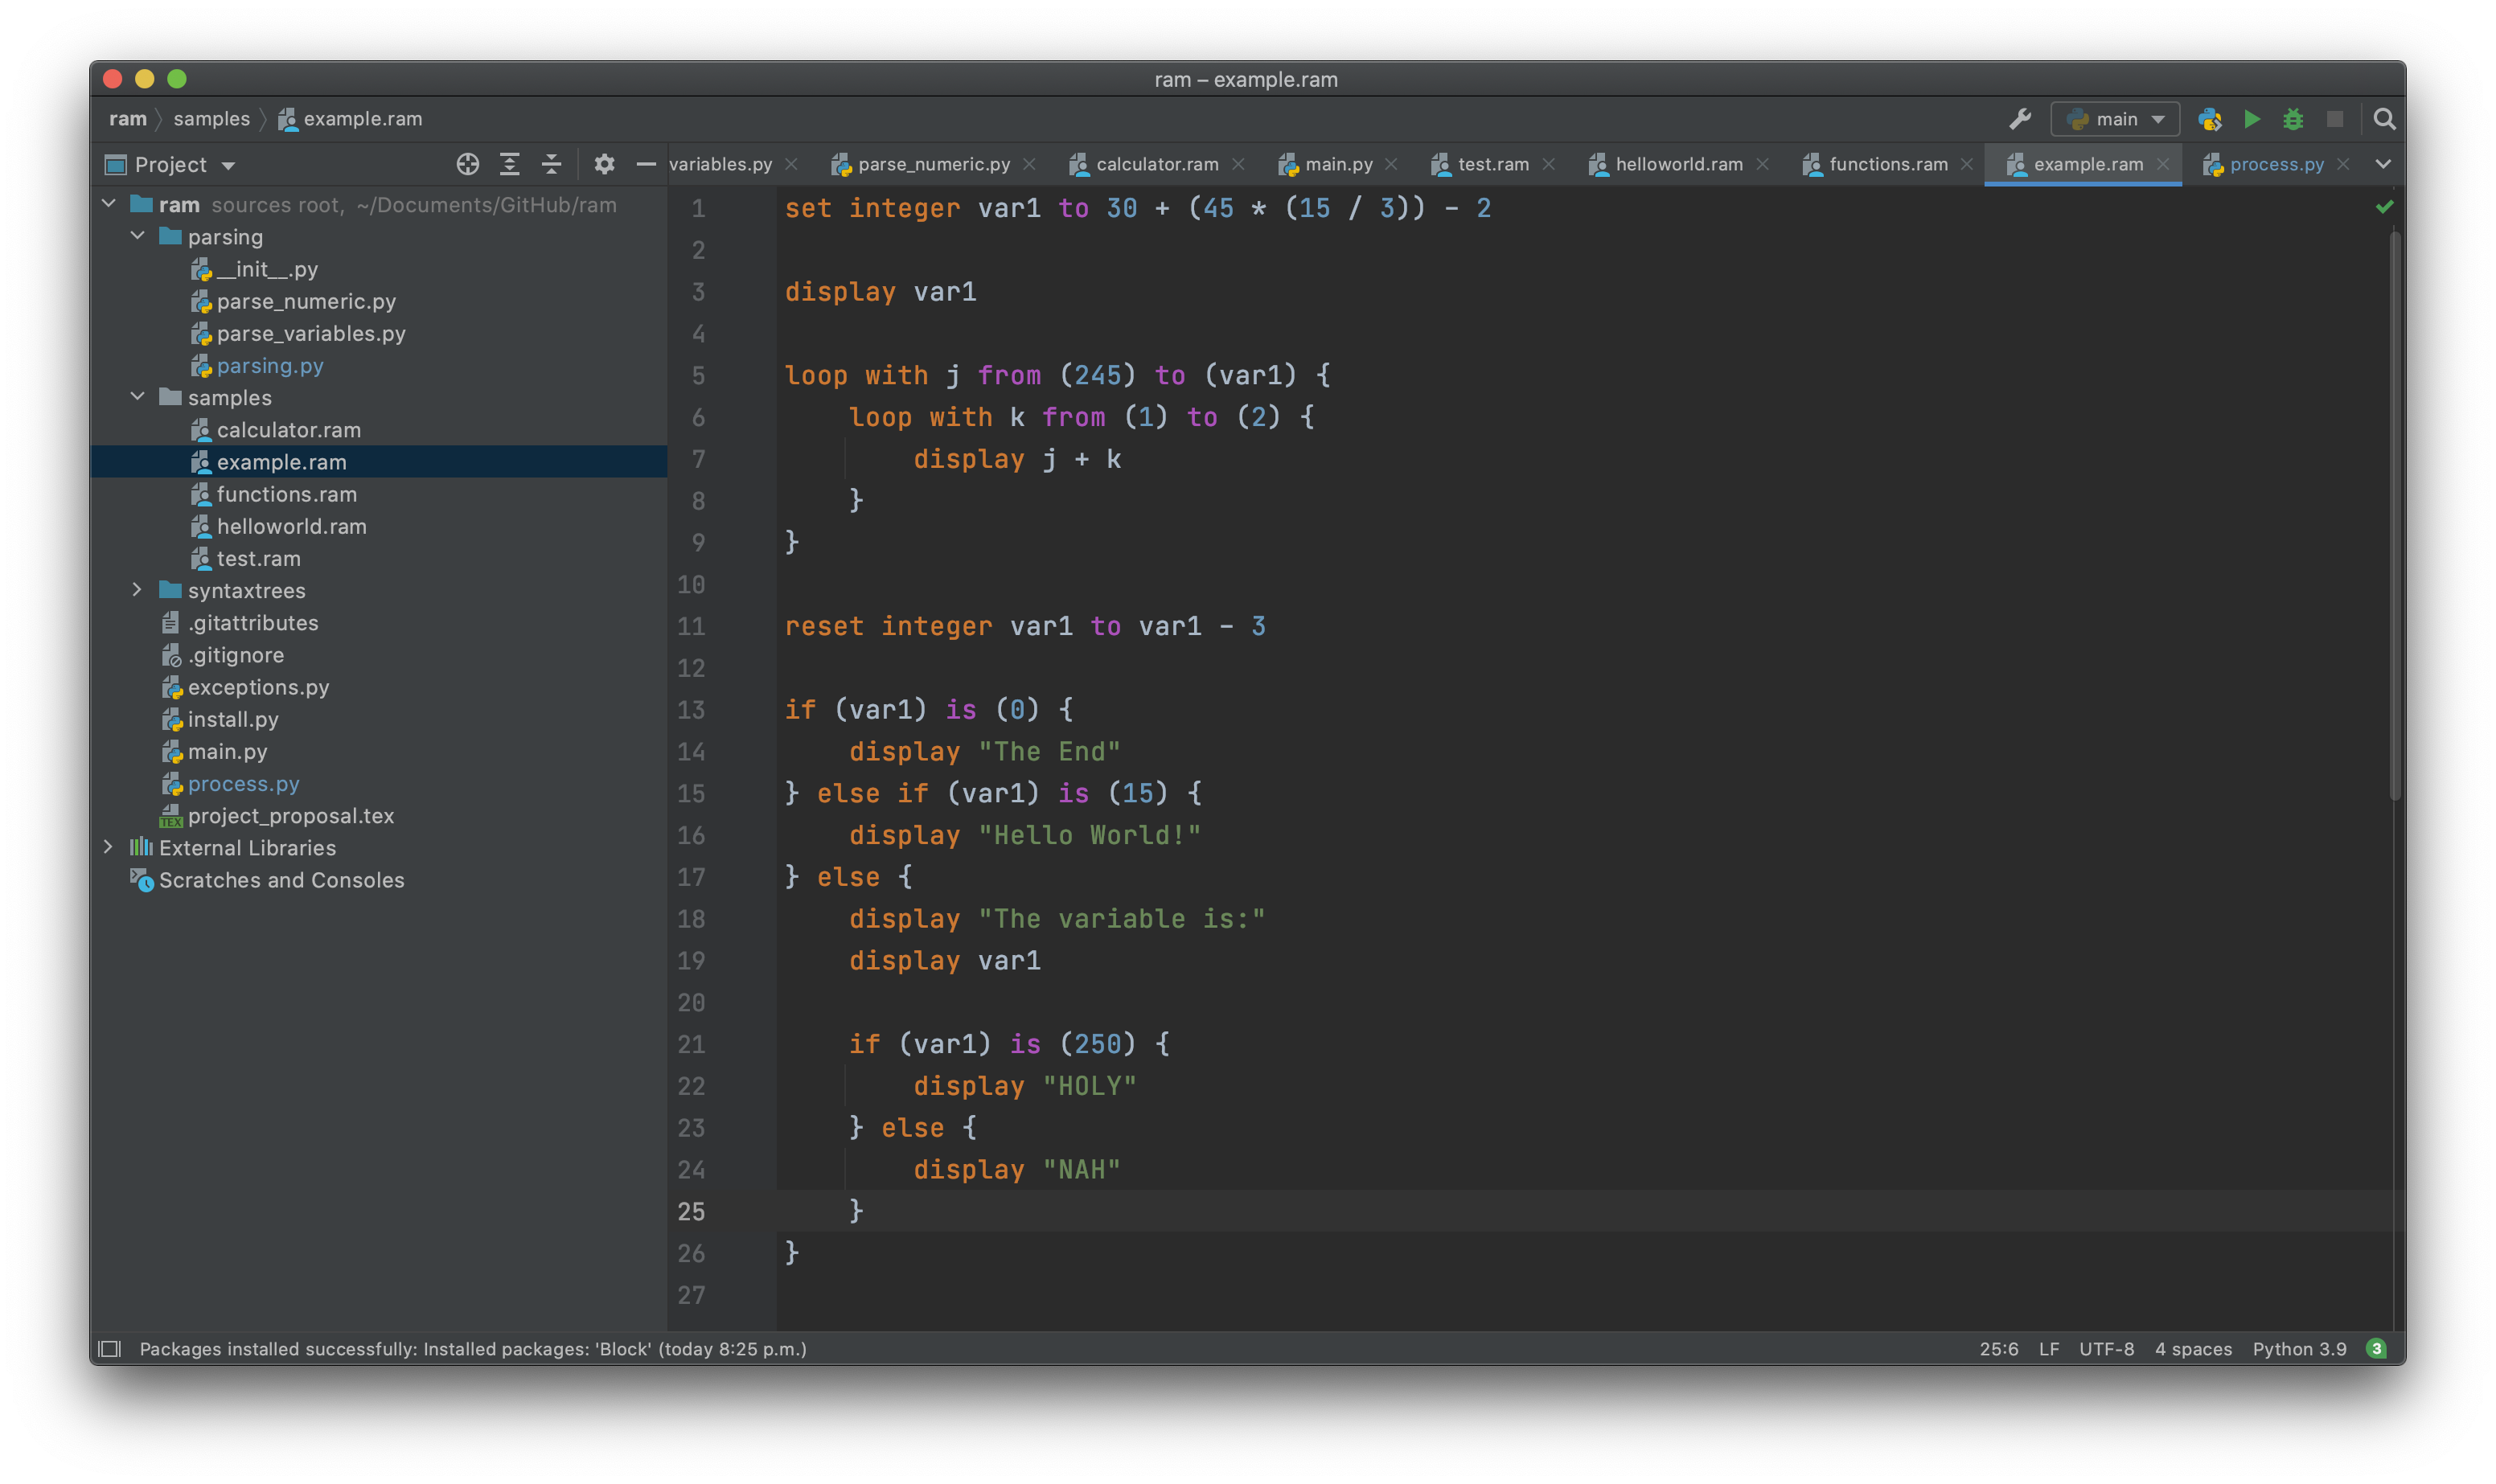
\includegraphics[scale=0.2]{terminal5.png}
            \end{center}
            
            \item Run main.py
            
            \item You will be prompted to enter the file path of the \texttt{.ram} file to run.
            
            \item The console runs the file!
        \end{itemize}
    \end{itemize} 

\subsection*{Technical Notes}

\begin{itemize}
    \item Strings must be defined with double quotes, not single quotes.
    
    \item Functions must have at least one parameter.
    
    \item Return statements, if any, must be the last line in a function.
    
    \item There cannot be spaces when calling functions (i.e. \texttt{f[x=40,y=50]}).
    
    \item The ending curly brace of a loop, function, or if statement must be the only item in the line.
    
    \item Arithmetic operators must be spaced out following a standard whitespace convention (i.e. \texttt{(1 + 3) * 5 / 2} instead of \texttt{(1 +3)* 5/2}).
    
    
    
\end{itemize}

\section*{Changes}

% Although the task at hand was difficult, our group knew that we could get it done. 
The project proposal provided a clear outline of our final objective, and we had an explicit plan to arrive at the final result. Despite no changes to our final objectives, we had to alter our computational plan in certain areas. In particular, we found that the libraries we had initially planned on integrating, \texttt{ast} and \texttt{nltk}, did not serve the intended purpose. We actually ended up hard-coding all of the ASTs, using some of the basic expressions included in the \emph{CSC111} Course Notes \cite{david}.

\section*{Discussion}

Upon testing numerous different sample files with many different variations of code --- a combination of assignment statements, loops, if statements, and functions --- we have discerned that our program is able to accurately take in the code as strings, and parse them to appropriate blocks. 

Referring back to our initial project goal, we see that we were able to successfully create a new programming language that is easily translatable to English and helps better prepare beginner programmers to use another programming language. The syntax that we had in mind was properly executed and properly reinforced. That is, when users do not correctly follow syntax requirements, the appropriate errors are raised. In addition, we built an extremely interactive environment where the user can do an array of things all the way from simple arithmetic calculations to building entire algorithms. It is very interesting to see the intricate and extremely nuanced approach to building a language. The process of going from strings to blocks of code which then gets parsed and interpreted by the system was expectantly difficult as a large majority of our key functions had especially complicated and technically demanding recursive implementations.

The limitations we encountered largely had to do with the sheer complexity of many of the key function implementations, alongside the general project as a whole. In addition to that, we feel that we were very ambitious in the early stages of our exploration process which minimized the time we had to implement our actual plan. Given an increase in the time restriction, we would've liked to see what additional features we could have integrated into the program from things like comments to nested functions. Given the nature of this project, whenever we encountered an error, it was very difficult to trace the error and determine what the triggers were. As a result, our approach for error testing was much more time consuming and unreliable than we had hoped for. 

To explore the content further, we may have tried to implement comments so that our users can potentially leave bits of information for their own reference. Alongside that, we could have tried to explore new libraries that could expand the range of possibilities. Lastly, we could have further investigated the possibilities of nested functions. 

\begin{thebibliography}{9}

\bibitem{david}
David Liu. \textit{CSC111 Lectures}. University of Toronto. 2021.

\bibitem{ASTs}
Dennis Howe. \textit{Free On-line Dictionary of Computing}. Internet Encyclopedia Project. 2008.

\bibitem{pyAST}
\textit{Abstract Syntax Trees}. Python Documentation. Available from: \link{https://docs.python.org/3/library/ast.html}

\bibitem{pyNLTK}
\textit{Natural Language Toolkit}. Python Documentation. Available from: \link{https://www.nltk.org/}

\bibitem{def}
Chapman, Nigel P. \textit{LR Parsing: Theory and Practice, Cambridge University Press}. 1987.

\end{thebibliography}

\end{document}